\chapter{Implémentation}
        \section{Choix des technologies} 
        \paragraph{} 
\begin{tabular}{|c|p{1.5cm}|p{2.7cm}|p{4cm}|}
        \hline
        Technologie & Version & Utilité & Raison du choix \\
        \hline
        Linux & Ubuntu 20.04.1 LTS & OS & Les trois membres utilisent Linux \\
        \hline
        Git/Github & 2.25.1 & Système de contrôle de version & Il permet de travailler à distance et en même temps et de garder une trace des différentes versions\\
        \hline 
        StarUml & 4.0.0 & Conception & Le choix de UML a été imposé par le client dès le départ. \\
        \hline 
        MySQL & 15.1 & SGBD & Open source | Facile à utiliser\\
        \hline 
        MySQL Workbench & 8.0 & Modélisation des données & Open source | Design Database sans code\\
        \hline
        PHP & 7.4.13 & Codage backend & Open source | Robuste | Sécurité | Imposé par le client\\
        \hline
\end{tabular}
\begin{tabular}{|c|p{1.5cm}|p{2.7cm}|p{4cm}|}
        \hline
        Laravel Framework & 8.15.0 & Programmation web & Prise en charge de l’architecture MVC | Facilite d’utilisation du Framework | Sécurité et performance | Documentation et communauté\\
        \hline
        HTML5 & 5 & Programmation structure frontend & Open source | Facilité\\
        \hline
        CSS3 & 3 & Programmation design frontend & Open source | Facilité\\
        \hline
        Bootstrap & 3.3.7 & Programmation design frontend & Open source | Facilité\\
        \hline
        Jquery & 3.1.2 & Programmation gestion des evenements frontend & Open source | Facilité\\
        \hline
        Google: Gmail API &  & SMTP & Server mail pour délivrer les email\\
        \hline
\end{tabular}

\section{La hiérarchie dans l'application}
\paragraph{}
Trois niveaux d'utilisation sont considérés au sein de l'application.
Chacun d'eux détient des privilèges en plus de celui qui vient directement après lui.
Les abonnés sont ceux qui peuvent poser le moins d'actions possibles dans le système. ils 
ne peuvent rien faire de plus que lire les données disponibles. De ce fait, 
ils peuvent voir tous les livres qui sont disponibles à chaque instant, et recevoir 
des notifications lorsqu'ils auront passé trop de temps avec un ouvrage en main.\par 
De leur côté, les bibliothécaires détiennent des droits de ressources matérielles. En plus
des droits d'accès des abonnés, ils peuvent agir sur les différents 
emprunts ainsi que que sur les données relatives aux ouvrages. \par 
Et enfin, le gestionnaire peut tout faire, et plus particulièrement gérer les 
utilisateurs du système.
\section{Interface utilisateur}
\paragraph{}       
L'interface utilisateur a été réfléchi de telle sorte que n'importe qui 
puisse se retrouver facilement sur l'application. Aucun téléchargement préalable n'est requis, de même 
qu'il ne sera pas du tout nécessaire de faire un cours complet pour expliquer à un nouvel utilisateur
les différentes utilités de chaque bouton.

\section{Diagrammes}
\subsection{Diagrammes des cas d'utilisation}
\paragraph{}
Ici, seront expliqués les différents cas d'utilisation que l'on peut retrouver au sein de 
l'application. D'abord, le cas général sera présenté, puis chaque cas particulier sera détaillé
et aura une image comme support.
\subsubsection{Cas d'utilisation général} 
\begin{figure}[h]
        \centering
        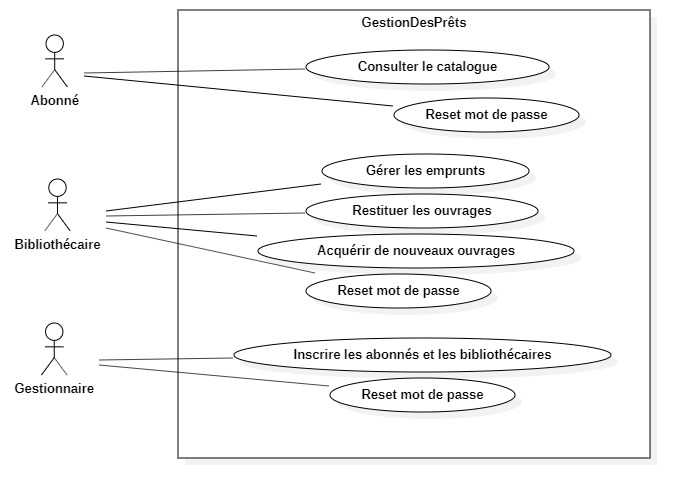
\includegraphics[width=1\textwidth]{generalUseCase}
        \caption{Diagramme des cas d'utilisation général}
        \label{image-generalUseCase}
        \end{figure}
\paragraph{}
De façon générale, l'objectif principal de l'application est d'assurer la 
gestion des prêts dans une bibliothèque universitaire. De ce fait, tois 
acteurs principaux sont à prendre en compte: l'abonné, le bibliothécaire et 
le gestionnaire. L'abonné est uniquement capable de consulter le catalogue.
Le bibliothécaire est, de son côté, responsable de gérer les emprunts, restituer les ouvrages et 
acquérir de nouveaux ouvrages. Et enfin, le gestionnaire a pour rôle d'inscrire de nouveaux utilisateurs
dans le système. Néanmoins, ces trois catégories peuvent à tout moment réinitialiser leur mot de passe ainsi 
que voir les activités qu'ils ont effectué en matière d'emprunts.

\subsubsection{Consultation du catalogue} 
\paragraph{}
\begin{figure}[h]
        \centering
        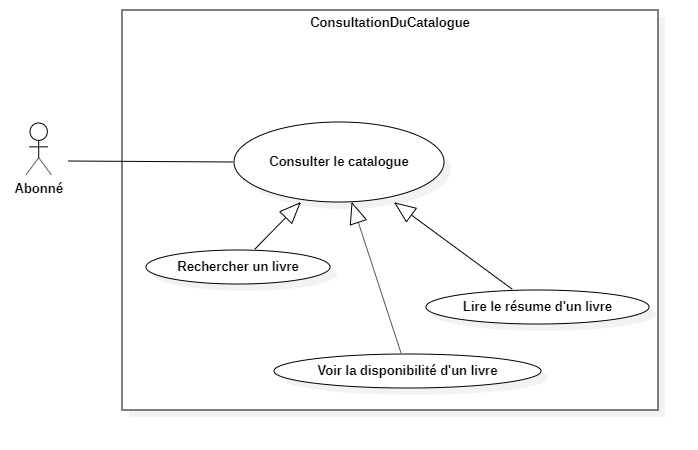
\includegraphics[width=1\textwidth]{consultationDuCatalogueUseCase}
        \caption{Diagramme du cas de consultation du catalogue}
        \label{image-consultationDuCatalogueUseCase}
        \end{figure}
\par
La consultation du catalogue est particulièrement réservée aux abonnés, même si 
tous les utilisateurs y ont accès. Cette activité évite à l'abonné un déplacement
inutile dans le cas où le livre souhaité ne serait pas disponible. \par 
Elle peut être décrite comme suit: \par 
\begin{tabular}{|c|p{7cm}|}
        \hline
        Titre & Consulter le catalogue  \\
        \hline
        Objectif & Permettre à l'utilisateur de vérifier la disponibilité d'un ouvrage \\
        \hline
        Acteur & Abonné \\
        \hline
        Précondition & \begin{itemize}
                \item L'abonné s'est authentifié 
        \end{itemize} \\
        \hline
        Postcondition & \begin{itemize}
                \item L'abonné peut voir le statut des différents livres
                \item L'abonné peut télécharger la liste des livres
        \end{itemize} \\
        \hline
        Fonctionnement Normal & \begin{itemize}
                \item L'abonné se rend sur le site
                \item Il s'authentifie
                \item Il a accès aux différents livres
        \end{itemize} \\
        \hline
        Exception & \begin{itemize}
                \item L'abonné n'a pas été enregistré sur le système - Il ne peut pas avoir accès à la plateforme; il 
                doit contacter le gestionnaire directement
        \end{itemize} \\
        \hline
\end{tabular}

\subsubsection{Acquisition des ouvrages}
\paragraph{} 
\begin{figure}[h]
        \centering
        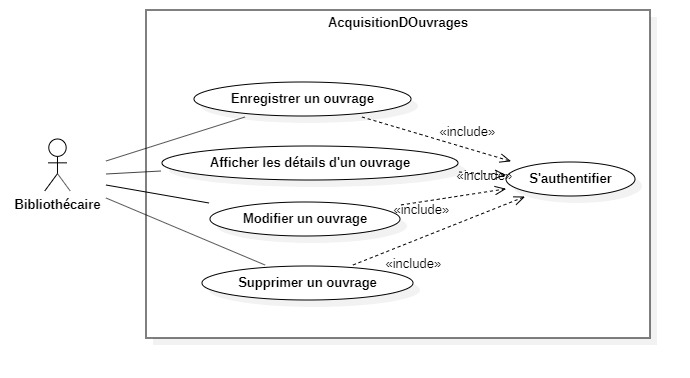
\includegraphics[width=1\textwidth]{acquisitionDesOuvragesUseCase}
        \caption{Diagramme du cas d'acquisition des ouvrages}
        \label{image-acquisitionDesOuvragesUseCase}
        \end{figure}
\par
L'acquisition des ouvrages est réservée plus principalement au bibliothécaire. Cette activité lui permet de garder à jour
la base de données à chaque nouvel arrivage de bouquins. Ceci permettra aux abonnées de savoir de quels livres dispose
la bibliothèque.  \par 
Elle peut être décrite comme suit: \par 
\begin{tabular}{|c|p{7cm}|}
        \hline
        Titre & Acquisition d'ouvrages  \\
        \hline
        Objectif & Permettre au biliothécaire d'enregistrer un nouvel ouvrage \\
        \hline
        Acteur & Bibliothécaire \\
        \hline
        Précondition & \begin{itemize}
                \item Le bibliothécaire s'est authentifié 
        \end{itemize} \\
        \hline
        Postcondition & \begin{itemize}
                \item Un nouvel ouvrage est enregistré dans la base de données
        \end{itemize} \\
        \hline
\end{tabular}
\par 
\begin{tabular}{|c|p{7cm}|}
        \hline
        Fonctionnement Normal & \begin{itemize}
                \item Le bibliothécaire se rend sur le site
                \item Il s'authentifie
                \item Il va dans le module "Livres"
                \item Il clique sur ajouter
                \item Il remplit les champs et fait sa sauvegarde
                \item Un message de succès est affiché
        \end{itemize} \\
        \hline
        Exception & \begin{itemize}
                \item Les champs obligatoires ne sont pas remplis - Un message d'erreur est affiché
                \item Une position a déjà été enregistrée - L'utilisateur en est signalé
        \end{itemize} \\
        \hline
\end{tabular}

\subsubsection{Gestion des emprunts} 
\paragraph{}
\begin{figure}[h]
        \centering
        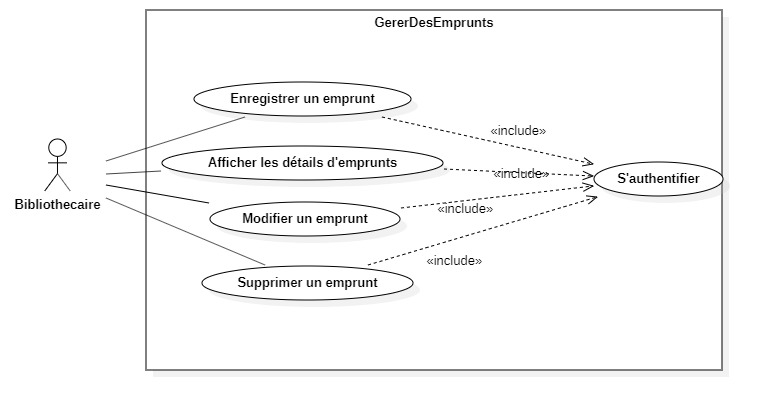
\includegraphics[width=1\textwidth]{gestionDesEmpruntsUseCase}
        \caption{Diagramme du cas de gestion des emprunts}
        \label{image-gestionDesEmpruntsUseCase}
        \end{figure}
\par
L'acteur direct de la gestion des emprunts n'est nul autre que le bibliothécaire. Cette activité 
permet au bibliothécaire d'enregistrer les informations nécessaires afin de retracer l'utilisation
des différents ouvrages.\par 
Elle peut être décrite comme suit: \par 
\begin{tabular}{|c|p{7cm}|}
        \hline
        Titre & Gérer des emprunts \\
        \hline
        Objectif & Permettre au bibliothécaire de faire différentes actions sur un prêt \\
        \hline
        Acteur & Bibliothécaire \\
        \hline
        Précondition & \begin{itemize}
                \item Le bibliothécaire s'est authentifié 
                \item L'abonné existe
                \item L'ouvrage existe
        \end{itemize} \\
        \hline
        Postcondition & \begin{itemize}
                \item L'emprunt est enregistré 
        \end{itemize} \\
        \hline
\end{tabular}
\par 
\begin{tabular}{|c|p{7cm}|}
        \hline
        Fonctionnement Normal & \begin{itemize}
                \item Le bibliothécaire se rend sur le site
                \item Il s'authentifie
                \item Il va dans le module "Emprunts"
                \item Il clique sur ajouter
                \item Il remplit les champs et fait sa sauvegarde
                \item Un message de succès est affiché
        \end{itemize} \\
        \hline
        Exception & \begin{itemize}
                \item L'abonné n'a pas été enregistré sur le système - Le bibliothécaire ne peut pas remplir le champ
                \item Le livre n'est pas enregistré dans la base de données - Le bibliothécaire ne peut pas remplir le champ
        \end{itemize} \\
        \hline
\end{tabular}


\subsubsection{Restitution des ouvrages} 
\paragraph{}
\begin{figure}[h]
        \centering
        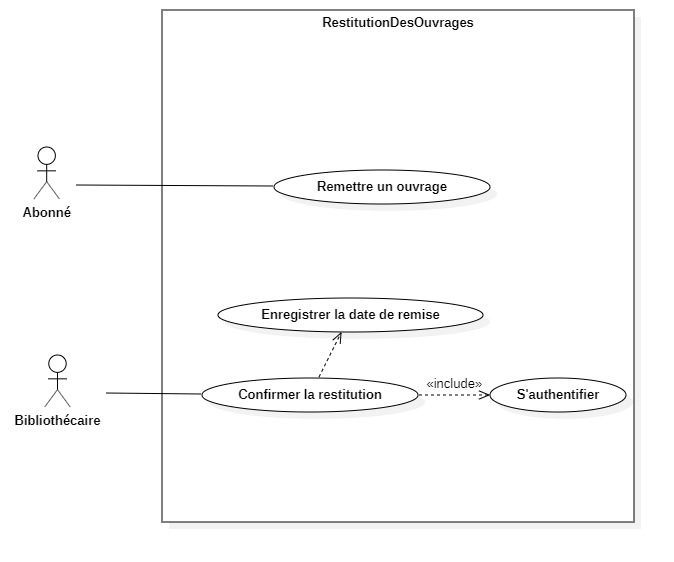
\includegraphics[width=1\textwidth]{restitutionDesOuvragesUseCase}
        \caption{Diagramme du cas de restitution des ouvrages}
        \label{image-restitutionDesOuvragesUseCase}
        \end{figure}
\par
Cette activité prend en compte tant l'abonné que le bibliothécaire. Elle permet de sauvegarder la 
date à laquelle un livre a été  rendu afin de déterminer s'il est disponible ou pas. \par 
Elle peut être décrite comme suit: \par 
\begin{tabular}{|c|p{7cm}|}
        \hline
        Titre & Restitution des ouvrages \\
        \hline
        Objectif & Permettre de se rappeler quand un livre a été rendu \\
        \hline
        Acteur & Abonné, Bibliothécaire \\
        \hline
        Précondition & \begin{itemize}
                \item Le bibliothécaire s'est authentifié 
                \item L'emprunt avait été enregistré
        \end{itemize} \\
        \hline
        Postcondition & \begin{itemize}
                \item Le livre est à nouveau disponible
        \end{itemize} \\
        \hline
\end{tabular}
\par 
\begin{tabular}{|c|p{7cm}|}
        \hline
        Fonctionnement Normal & \begin{itemize}
                \item L'abonné se rend à la bibliothèque avec le livre
                \item Le gestionnaire va sur le site
                \item Il s'authentifie
                \item Il va dans le module "Emprunts"
                \item Il cherche l'emprunt en question pour le modifier
                \item Il ajoute la date de restitution
                \item Un message de succès est affiché
        \end{itemize} \\
        \hline
        Exception & \begin{itemize}
                \item 
        \end{itemize} \\
        \hline
\end{tabular}

\subsubsection{Gestion des utilisateurs} 
\paragraph{}
\begin{figure}[h]
        \centering
        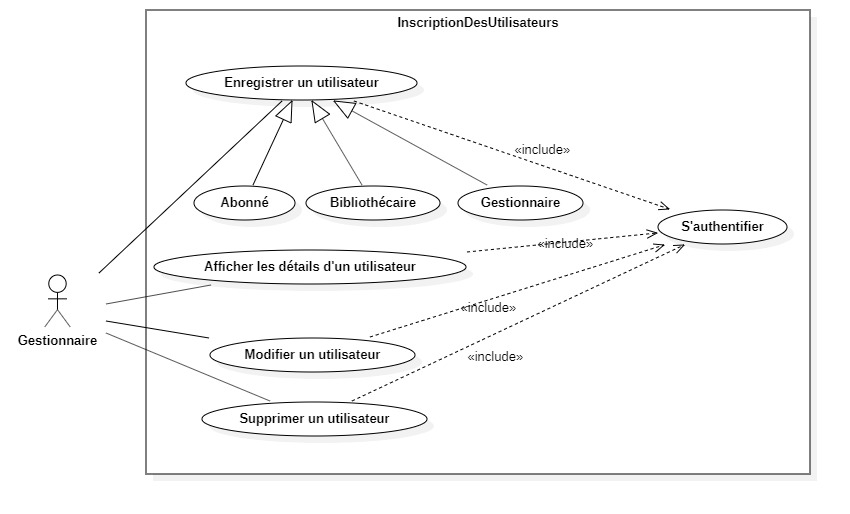
\includegraphics[width=1\textwidth]{gestionDesUtilisateursUseCase}
        \caption{Diagramme du cas de gestion des utilisateurs}
        \label{image-gestionDesUtilisateursUseCase}
        \end{figure}
\par 
L'unique utilisateur à avoir accès à ce type de gestion est l'administrateur. Dans 
ce cas de figure précis, il s'agit du gestionnaire. Cette activité 
permet d'enregistrer les informations relatives à chaque utilisateur. \par 
Elle peut être décrite comme suit: \par 
\begin{tabular}{|c|p{7cm}|}
        \hline
        Titre & Inscription des utilisateurs \\
        \hline
        Objectif & Permettre au gestionnaire de faire différentes actions sur les données d'un utilisateur \\
        \hline
        Acteur & Gestionnaire \\
        \hline
        Précondition & \begin{itemize}
                \item Le gestionnaire s'est authentifié 
        \end{itemize} \\
        \hline
        Postcondition & \begin{itemize}
                \item L'utilisateur est enregistré 
        \end{itemize} \\
        \hline
\end{tabular}
\par 
\begin{tabular}{|c|p{7cm}|}
        \hline
        Fonctionnement Normal & \begin{itemize}
                \item Le gestionnaire se rend sur le site
                \item Il s'authentifie
                \item Il va dans le module "Utilisateurs"
                \item Il clique sur ajouter
                \item Il remplit les champs et fait sa sauvegarde
                \item Un message de succès est affiché
        \end{itemize} \\
        \hline
        Exception & \begin{itemize}
                \item Les champs obligatoires ne sont pas remplis - Un message d'erreur est affiché
                \item Une information unique est répliquée - Un message d'erreur est affiché
                \item Les mots de passe ne sont pas identiques - Un message d'erreur est affiché
        \end{itemize} \\
        \hline
\end{tabular}

\subsection{Diagrammes de séquence}
\paragraph{} 
Les diagrammes de séquence sont utiles pour permettre la représentation des interactions 
entre les différents acteurs et le système dans un ordre chronologique.
\subsubsection{Acquisition des ouvrages} 
\paragraph{}
\begin{figure}[h]
        \centering
        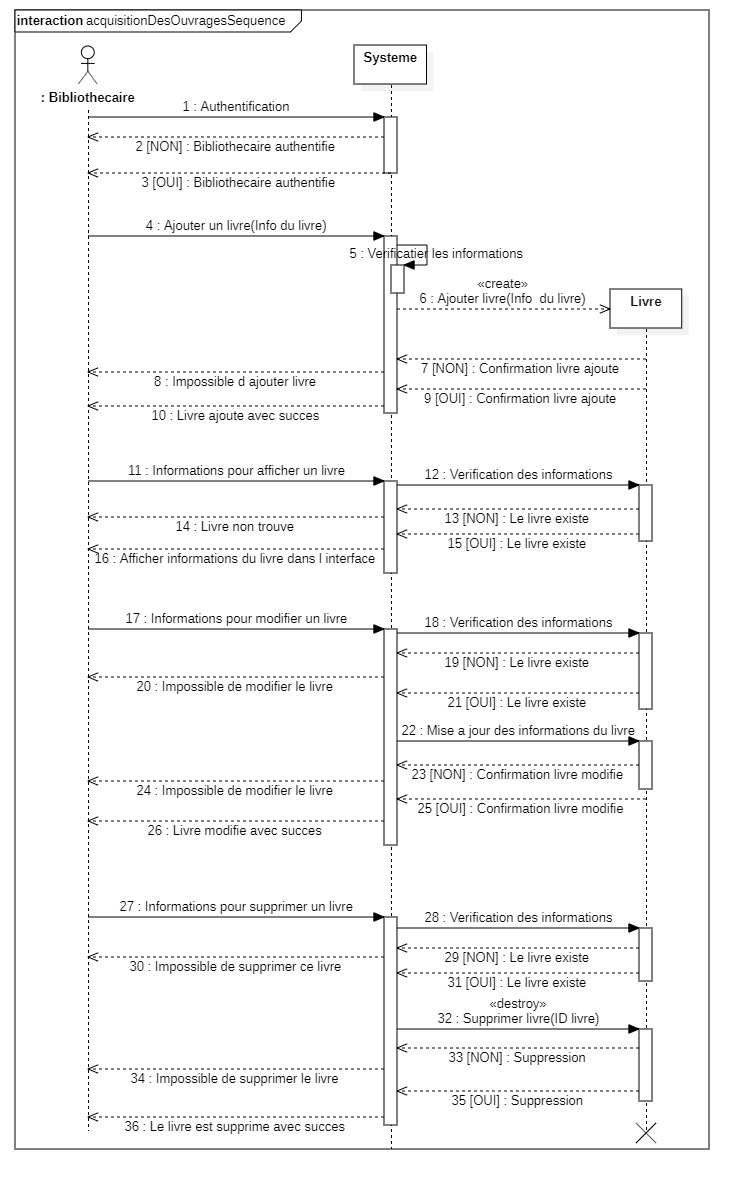
\includegraphics[width=0.6\textwidth]{acquisitionDesOuvragesSequence}
        \caption{Diagramme de séquence pour l'acquisition des ouvrages}
        \label{image-acquisitionDesOuvragesSequence}
        \end{figure}
\par
Pour commencer, il faut que le bibliothécaire s'authentifie sur le système.
Une fois l'authentification réussie, il peut alors rentrer les données dans le système.
Les données sont analysées et le bibliothécaire peut enfin valider la sauvegarde 
lorsque toutes les informations ont été bien rentrées. \par 
Si le bibliothécaire souhaite afficher les informations relatives à un livre, il doit d'abord 
être authentifié. Puis il cherche/recherche le livre en question afin d'avoir accès aux 
différentes informations. Le système vérifie alors les informations pour s'assurer que 
le livre existe avant d'en afficher toutes les informations y relatives. \par 
Le bibliothécaire a aussi le pouvoir de modifier les informations liées à un ouvrage.
Encore une fois, il ne peut rien faire sans être authentifié. Tout comme pour l'affichage, 
il cherche le livre désiré pour ensuite le modifier cette fois. Une fois la modification 
réussie, un message de succès est affiché. Si la modification n'est pas réussie, au 
contraire, un message d'erreur fait son apparition. \par 
Et enfin, le bibliothécaire peut supprimer un livre. Au cours de cette suppression, le livre
devient inaccessible au niveau de l'application, mais il reste disponible dans la base de 
données afin que toute action futur soit encore possible. \par
\subsubsection{Consultation du catalogue} 
\paragraph{}
\begin{figure}[h]
        \centering
        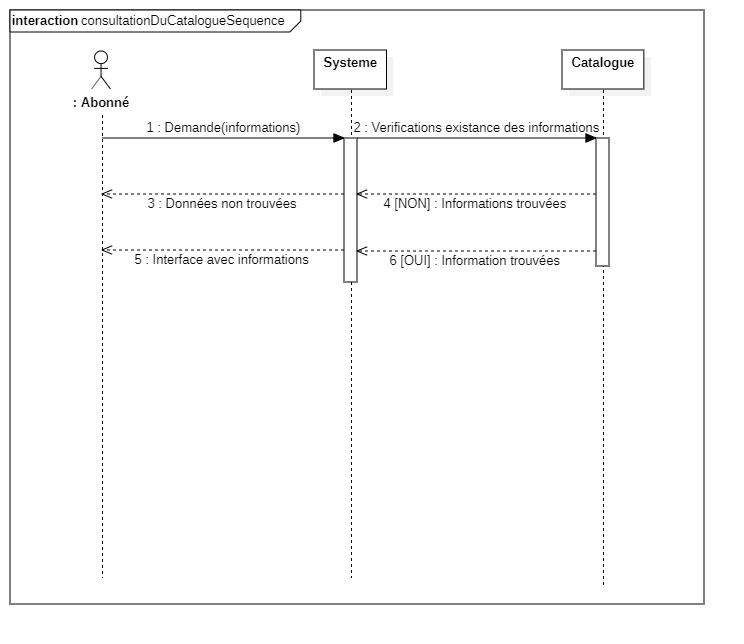
\includegraphics[width=1\textwidth]{consultationDuCatalogueSequence}
        \caption{Diagramme de séquence pour la consultation du catalogue}
        \label{image-consultationDuCatalogueSequence}
        \end{figure}
\par 
Lors de la consultation du cataloque, tout intéressé peut faire de la lèche-vitrine à 
sa guise. Mais si un abonné veut vérifier la disponibilité d'un ouvrage, il doit 
obligatoirement s'authentifier. Il donc chercher/rechercher l'ouvrage qu'il lui faut, et le 
système prend le soin d'afficher le résultat de ses recherches.
\subsubsection{Gestion des utilisateurs} 
\paragraph{}
\begin{figure}[h]
        \centering
        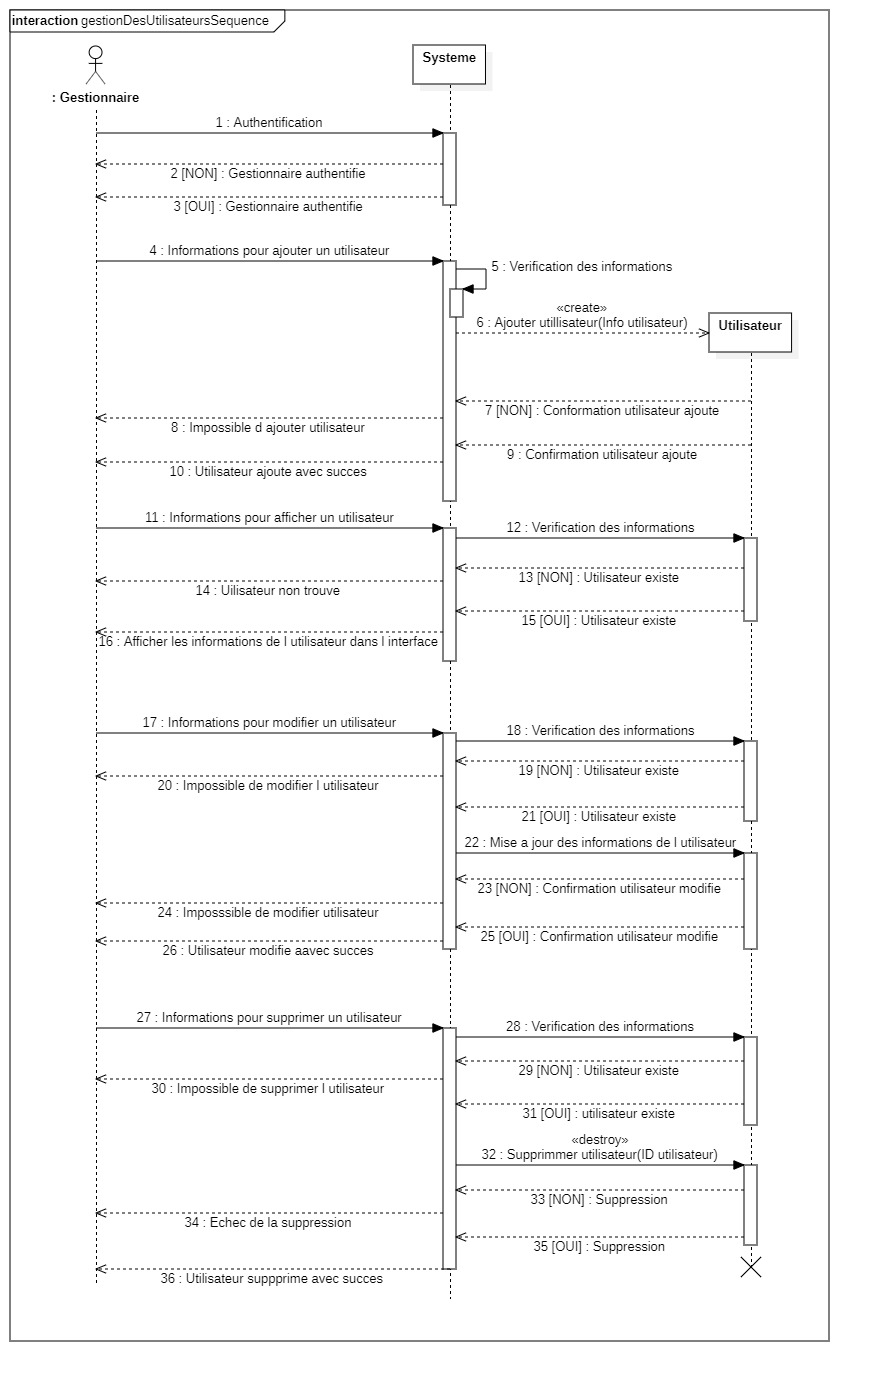
\includegraphics[width=0.5\textwidth]{gestionDesUtilisateursSequence}
        \caption{Diagramme de séquence pour la gestion des utilisateurs}
        \label{image-gestionDesUtilisateursSequence}
        \end{figure}
\par
Quelle que soit l'action que désire entamer le gestionnaire, il doit avant tout s'authentifier
en tant que tel. S'il doit ajouter un nouvel utilisateur, il lui suffira, par la suite 
d'enregistrer les informations dans les champs dédiés à cette fin. À son tour, le système 
vérifie les informations avant de laisser le soin au gestionnaire de valider la sauvegarde.
Une fois réussie, l'utilisateur est alors enregistré et pourra s'authentifier sur le 
système. \par 
Les étapes de modification, d'affichage et de suppression d'un utilisateur ne diffèrent 
pas de celles expliquées plus tôt dans le cas de la gestion des ouvrages. Les détails 
peuvent ainsi se passer de présentation; le même modèle est à suivre.
\subsubsection{Restitution des ouvrages} 
\paragraph{}
\begin{figure}[h]
        \centering
        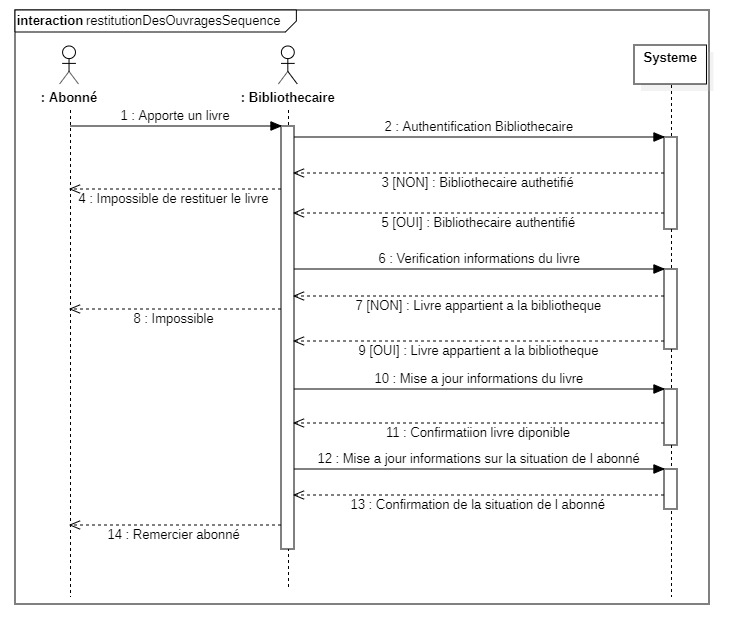
\includegraphics[width=1\textwidth]{restitutionDesOuvragesSequence}
        \caption{Diagramme de séquence pour la restitution des ouvrages}
        \label{image-restitutionDesOuvragesSequence}
        \end{figure}
\par
Pour restituer un ouvrage, l'abonné se présente sur place. Pour assurer le suivi, le 
bibliothécaire doit d'abord s'authentifier. Il va ensuite dans le module des emprunts 
et cherche le correspondant à celui recherché. Il ajoute alors la date de restitution,
ce qui fait passer automatiquement le statut de l'ouvrage de "Non disponible" à disponible.
Le livre est donc rendu et l'abonné peut partir ou exécuter autant de nouveaux emprunts
que le lui permet son quota.
\subsubsection{Gestion des emprunts} 
\paragraph{}
\begin{figure}[h]
        \centering
        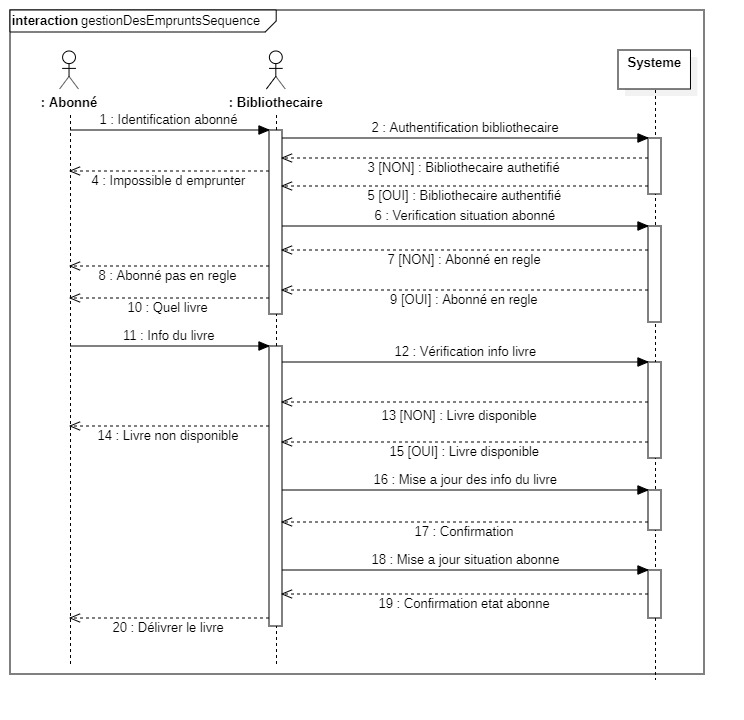
\includegraphics[width=1\textwidth]{gestionDesEmpruntsSequence}
        \caption{Diagramme de séquence pour la gestion des emprunts}
        \label{image-gestionDesEmpruntsSequence}
        \end{figure}
\par
La première étape consiste en la présentation de l'abonné à la bibliothèque afin de 
faire un emprunt. Puis, le responsable s'authentifie pour faire le suivi nécessaire. Avant 
tout, il doit s'assurer que cet abonné existe dans le système. Si tel n'est pas le cas, le 
gestionnaire est le seul capable de l'enregistrer. Une fois l'abonné validé, le 
bibliothécaire peut remplir les champs requis pour l'enregistrement d'un emprunt. Seuls 
les livres disponibles à l'instant seront affichés pour faciliter la sélection des choix.
Si l'abonné détient encore trois livres qu'il n'a jamaias restitué, un message d'erreur 
est affiché et il ne pourra effectuer tant qu'il ne les aura pas rendus. Si tout est 
correct, l'enregistrement est validé et l'abonné peut partir sans contrainte.

\subsection{Diagrammes de ce qu'on n'a pas demande}
\paragraph{} 
Lorem ipsum dolor sit amet, consectetur adipiscing elit. Mauris at ultrices purus. Donec finibus metus et augue sodales posuere. Proin sit amet turpis dictum, iaculis felis in, scelerisque massa. Nullam aliquam nunc eget fringilla volutpat. Integer et mauris et massa imperdiet scelerisque mollis at sapien. Donec condimentum felis eget sagittis ultricies. Nunc laoreet augue id consectetur vulputate. Cras sagittis aliquam risus sit amet tempus. Curabitur finibus neque eget magna efficitur, sed dignissim quam sagittis. Ut euismod justo id gravida pulvinar. Ut urna magna, auctor maximus volutpat ac, elementum sed mi.
